\documentclass[12pt,a4paper]{article}

% ── Packages ──────────────────────────────────────────────────────────────────
\usepackage[utf8]{inputenc}
\usepackage[T1]{fontenc}
\usepackage[margin=2.5cm]{geometry}
\usepackage{hyperref}
\usepackage{graphicx}
\usepackage{listings}
\usepackage{xcolor}
\usepackage{tikz}
\usetikzlibrary{shapes.geometric, arrows.meta, positioning}
\usepackage{booktabs}
\usepackage{parskip}
\usepackage{microtype}
\usepackage{lmodern}
\usepackage{amsmath}

% ── Code listing style ─────────────────────────────────────────────────────────
\definecolor{codebg}{HTML}{F5F5F5}
\definecolor{keyword}{HTML}{0000CC}
\definecolor{comment}{HTML}{008000}
\definecolor{string}{HTML}{CC0000}

\lstdefinestyle{java}{
  language=Java,
  backgroundcolor=\color{codebg},
  basicstyle=\ttfamily\small,
  keywordstyle=\color{keyword}\bfseries,
  commentstyle=\color{comment}\itshape,
  stringstyle=\color{string},
  numbers=left,
  numberstyle=\tiny\color{gray},
  numbersep=8pt,
  frame=single,
  framerule=0.4pt,
  rulecolor=\color{gray!40},
  breaklines=true,
  captionpos=b,
  tabsize=4,
  showstringspaces=false,
}
\lstset{style=java}

% ── Metadata ───────────────────────────────────────────────────────────────────
\title{%
  \textbf{SameGame in Java}\\[0.4em]
  \large An Object-Oriented Implementation Using the MVC and Observer Patterns\\[0.2em]
  \normalsize Object-Oriented Programming --- Project Report
}
\author{%
  Hayat Aodi, Erwann Lanteri-Enée, Rawan Meselmini, Salam Mohammad\\[0.4em]
  \normalsize Group 8
}
\date{May 2026 \\ Halmstad University}

% ══════════════════════════════════════════════════════════════════════════════
\begin{document}
\maketitle
\tableofcontents
\newpage

% ══════════════════════════════════════════════════════════════════════════════
\section{Introduction}
\label{sec:intro}

SameGame is a classic single-player puzzle game originally released in 1985.
The player is presented with a rectangular grid of coloured tiles.
A \emph{group} is a set of two or more tiles that share the same colour and are
connected through horizontal or vertical adjacency (four-directional, never
diagonal).
Clicking a valid group removes all tiles in it, awards points, and causes the
remaining tiles to fall downward under gravity; wholly empty columns then
collapse to the left.
The game ends when no valid group remains: if the board is completely empty the
player wins, otherwise the player loses.

The project required producing a fully functional Java implementation of this
game together with a clean, extensible design.
The specific decisions taken here were:

\begin{itemize}
  \item Use the \textbf{Model-View-Controller (MVC)} architectural pattern to
        separate game logic from rendering and input.
  \item Use the \textbf{Observer} pattern to decouple the model from its views,
        allowing multiple simultaneous renderers.
  \item Provide a \textbf{Swing GUI} as the primary view and a lightweight
        \textbf{console (ASCII) view} for debugging alongside it.
  \item Score groups with the quadratic formula $S = (n-2)^2$, rewarding
        larger groups disproportionately.
\end{itemize}

Similar games such as \emph{Bejeweled} or \emph{Candy Crush} involve
swapping adjacent tiles; SameGame is simpler in that only grouped removal
occurs, making it a good fit for a semester-length project without sacrificing
interesting design problems.
The implementation covers all standard rules and adds a hover-highlight
feature that previews which tiles will be removed before the player commits to
a click.

% ══════════════════════════════════════════════════════════════════════════════
\section{Design}
\label{sec:design}

\subsection{Architectural overview}

The program is organised into five Java packages whose dependency graph is
strictly layered: \texttt{observer} $\leftarrow$ \texttt{model} $\leftarrow$
\texttt{view} / \texttt{controller} $\leftarrow$ \texttt{Main}.
No lower-level package imports a higher-level one; in particular, \texttt{model}
contains zero references to \texttt{javax.swing} or any view class.

\begin{figure}[ht]
\centering
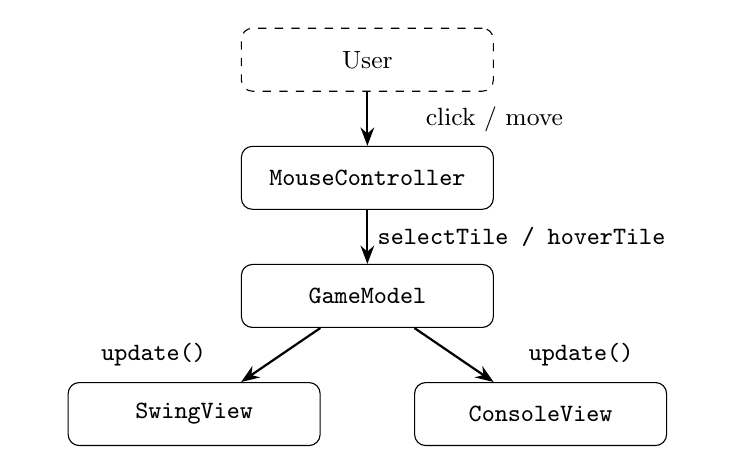
\begin{tikzpicture}[
  every node/.style={draw, rounded corners, minimum width=3.2cm,
                     minimum height=0.8cm, align=center, font=\small},
  arr/.style={-Stealth, thick}
]
  \node (user)  at (0,  4)   [dashed] {User};
  \node (ctrl)  at (0,  2.5) {\texttt{MouseController}};
  \node (model) at (0,  1)   {\texttt{GameModel}};
  \node (swing) at (-2.2, -0.5) {\texttt{SwingView}};
  \node (cons)  at ( 2.2, -0.5) {\texttt{ConsoleView}};

  \draw[arr] (user)  -- (ctrl)  node[midway, right, draw=none] {click / move};
  \draw[arr] (ctrl)  -- (model) node[midway, right, draw=none]
             {\texttt{selectTile / hoverTile}};
  \draw[arr] (model) -- (swing) node[midway, left,  draw=none]
             {\texttt{update()}};
  \draw[arr] (model) -- (cons)  node[midway, right, draw=none]
             {\texttt{update()}};
\end{tikzpicture}
\caption{Data-flow diagram for a single user interaction.}
\label{fig:dataflow}
\end{figure}

\subsection{Observer pattern}

Two interfaces in the \texttt{observer} package define the pattern contract:

\begin{description}
  \item[\texttt{GameSubject}] declares \texttt{addObserver},
        \texttt{removeObserver}, and \texttt{notifyObservers}.
        \texttt{GameModel} implements it.
  \item[\texttt{GameObserver}] declares a single method \texttt{update(GameModel)}.
        Both \texttt{SwingView} and \texttt{ConsoleView} implement it (via
        \texttt{GameView}, which extends \texttt{GameObserver} with lifecycle
        methods \texttt{display()} and \texttt{close()}).
\end{description}

The separation of \texttt{GameSubject} from \texttt{GameModel} means that
any code that only needs to register observers can depend on the interface
rather than the concrete class, limiting coupling.

\subsection{Model layer}

\texttt{GameModel} owns three pieces of mutable state: the \texttt{Board},
an integer score, and a \texttt{GameState} enum (\texttt{PLAYING},
\texttt{WIN}, \texttt{LOSE}).
It also stores the \emph{highlighted group}, a list of \texttt{int[]\{row,col\}}
pairs that represent the tile group under the cursor; this is updated by
\texttt{hoverTile()} and consumed by the view to paint a preview.

\texttt{Board} holds the two-dimensional \texttt{Tile[][]} grid and implements
three algorithms:

\begin{enumerate}
  \item \textbf{Flood-fill} (\texttt{findGroup}): a recursive depth-first search
        that collects all four-directionally connected tiles of the same colour
        starting from a seed position.
  \item \textbf{Gravity} (\texttt{applyGravity}): after removal, each column is
        compacted bottom-up so non-empty tiles slide down to fill gaps.
  \item \textbf{Column collapse} (\texttt{collapseColumns}): columns whose
        bottom cell is empty are removed and remaining columns shift left.
\end{enumerate}

\texttt{Tile} is a simple mutable value object holding a colour integer
(0 = empty, 1–\(N\) = game colour).
Mutability is intentional: \texttt{Board} sets colour to 0 in-place during
gravity and collapse rather than reallocating the entire grid.

\subsection{View layer}

Both views are \emph{passive}: they read state from the model reference passed
in \texttt{update()} but never mutate it.
\texttt{SwingView} uses a custom inner class \texttt{BoardPanel} (\texttt{JPanel})
for painting.
To avoid a circular import between the \texttt{view} and \texttt{controller}
packages, \texttt{SwingView} exposes \texttt{getBoardComponent()}, which returns
the board panel as a \texttt{JComponent}.
The controller attaches its listeners to this component without needing to
import the concrete \texttt{SwingView} type in the listener code.

\subsection{Controller layer}

\texttt{GameController} is an interface with two lifecycle methods,
\texttt{attach()} and \texttt{detach()}.
\texttt{MouseController} extends \texttt{MouseAdapter} (overriding only
\texttt{mouseClicked} and \texttt{mouseMoved}) and implements
\texttt{GameController}.
Pixel-to-grid conversion uses the constant \texttt{SwingView.TILE\_SIZE}:

\[
  \text{col} = \lfloor x_{\text{px}} / \texttt{TILE\_SIZE} \rfloor, \quad
  \text{row} = \lfloor y_{\text{px}} / \texttt{TILE\_SIZE} \rfloor
\]

A new input method (keyboard, network, etc.) requires only implementing
\texttt{GameController} and registering it in \texttt{Main}; no other class
changes.

% ══════════════════════════════════════════════════════════════════════════════
\section{Testing}
\label{sec:testing}

Testing was split into two complementary strategies.

\subsection{Automated unit tests}

JUnit 4 tests in \texttt{GameModelTest} cover the most critical model
invariants, since the model is the layer with no external dependencies.

\begin{lstlisting}[caption={Excerpt from \texttt{GameModelTest.java}},
                   label={lst:tests}]
@Test
public void testInitialScoreIsZero() {
    GameModel model = new GameModel(3);
    assertEquals(0, model.getScore());
}

@Test
public void testGameStartsPlaying() {
    GameModel model = new GameModel(3);
    assertEquals(GameState.PLAYING, model.getState());
}

@Test
public void testRestartResetsScore() {
    GameModel model = new GameModel(3);
    model.restart(3);
    assertEquals(0, model.getScore());
}
\end{lstlisting}

The tests verify:
\begin{itemize}
  \item Initial score is zero after construction.
  \item Initial game state is \texttt{PLAYING}.
  \item Calling \texttt{restart()} resets the score to zero.
\end{itemize}

\subsection{Manual integration testing}

Because \texttt{SwingView} depends on the Swing event dispatch thread, the
GUI layer was tested manually:

\begin{enumerate}
  \item Verified that clicking a single isolated tile (group size 1) has no
        effect on score or board state.
  \item Verified that clicking a group of \(n\) tiles increases the score by
        exactly $(n-2)^2$.
  \item Verified gravity: after removal, tiles above the gap fall to the bottom
        of their column with correct relative order.
  \item Verified column collapse: a column cleared entirely disappears and the
        columns to its right shift left.
  \item Verified end conditions: the win overlay appeared when the last group
        was removed; the lose overlay appeared when no valid moves remained.
  \item Verified the hover preview by moving the mouse over groups of varying
        sizes.
\end{enumerate}

% ══════════════════════════════════════════════════════════════════════════════
\section{Implementation Highlights}
\label{sec:highlights}

\subsection{Flood-fill group detection}

The flood-fill in \texttt{Board.findGroup} is a recursive depth-first search.
A key design choice was to return a \emph{list} of positions rather than
mutating the board in-place: the caller (\texttt{GameModel}) uses the same
list for both scoring and the hover-preview highlight before any tile is
actually removed.

\begin{lstlisting}[caption={Recursive flood-fill in \texttt{Board.java}},
                   label={lst:floodfill}]
private void floodFill(int r, int c, int color,
                       boolean[][] visited, List<int[]> group) {
    if (r < 0 || r >= rows || c < 0 || c >= cols) return;
    if (visited[r][c] || grid[r][c].getColor() != color) return;
    visited[r][c] = true;
    group.add(new int[]{r, c});
    floodFill(r - 1, c, color, visited, group);
    floodFill(r + 1, c, color, visited, group);
    floodFill(r, c - 1, color, visited, group);
    floodFill(r, c + 1, color, visited, group);
}
\end{lstlisting}

The \texttt{visited} array prevents the recursion from re-entering cells and
bounds-checking is done at the top of each call, keeping the main logic clean.

\subsection{Decoupling view and controller}

A subtle problem arises with MVC in Swing: the controller needs to attach a
\texttt{MouseListener} to the board panel, but if \texttt{MouseController}
imports \texttt{SwingView} it creates a dependency from
\texttt{controller} to \texttt{view}.
The chosen solution was to expose the panel through the \texttt{JComponent}
supertype:

\begin{lstlisting}[caption={\texttt{SwingView.getBoardComponent()} breaks the cycle},
                   label={lst:decouple}]
// In SwingView (view package)
public JComponent getBoardComponent() { return boardPanel; }

// In MouseController (controller package)
public void attach() {
    JComponent board = view.getBoardComponent();
    board.addMouseListener(this);
    board.addMouseMotionListener(this);
}
\end{lstlisting}

Both packages depend only on \texttt{javax.swing.JComponent}; neither creates
a dependency on the other's concrete type at the listener-registration site.

\subsection{Hover preview without extra state}

The hover preview reuses the same flood-fill path as a real click.
\texttt{GameModel.hoverTile()} stores the resulting group in
\texttt{highlightedGroup}; \texttt{SwingView.BoardPanel.paintComponent()}
reads it during every repaint and brightens those tiles.
No separate ``preview'' state was introduced; the model's highlighted-group
field doubles as the preview channel at zero extra cost.

% ══════════════════════════════════════════════════════════════════════════════
\section{Results and Evaluation}
\label{sec:results}

\subsection{Functionality}

All specified requirements were implemented:

\begin{itemize}
  \item Four-directional group detection with flood-fill.
  \item Quadratic scoring: $S = (n-2)^2$.
  \item Gravity and column collapse after each removal.
  \item Win / lose detection after every move.
  \item Hover-preview highlight before committing a click.
  \item Restart button that resets score and generates a new board.
  \item Parallel \texttt{ConsoleView} for debugging.
\end{itemize}

\subsection{Extensibility}

The MVC + Observer design makes the most common extensions straightforward:

\begin{description}
  \item[New view] Implement \texttt{GameView} and call
        \texttt{model.addObserver(newView)} in \texttt{Main}.
        No changes to any existing class.
  \item[New controller] Implement \texttt{GameController}, call
        \texttt{attach()} in \texttt{Main}.
        A keyboard controller, for example, would require zero changes to
        the model or views.
  \item[Board configuration] Change \texttt{GameModel.ROWS}, \texttt{COLS}, or
        pass a different \texttt{numColors} value; no other changes needed.
\end{description}

\subsection{Limitations}

\begin{itemize}
  \item No persistent high-score storage; the score resets on every run.
  \item Board size is fixed at compile time via constants rather than being
        configurable at runtime through a settings dialog.
  \item Deep flood-fills on large boards could overflow the call stack;
        an iterative implementation using an explicit \texttt{Deque} would
        be more robust.
\end{itemize}

% ══════════════════════════════════════════════════════════════════════════════
\section{Version Control}
\label{sec:git}

All development was tracked with Git.
The working tree followed a single linear branch (\texttt{main}) with commits
at meaningful milestones:

\begin{center}
\begin{tabular}{@{}ll@{}}
\toprule
\textbf{Hash} & \textbf{Message} \\
\midrule
\texttt{99e1277} & Init project \\
\texttt{dd98aaa} & SameGame V0 \\
\texttt{ff29a8e} & Add HOW\_TO\_RUN.md for project setup and execution \\
\texttt{dca12df} & Updated SameGame project and added design improvements \\
\texttt{8df6f57} & Updated Board.java \\
\texttt{0155159} & Updated test \\
\texttt{10e3440} & Updated \\
\bottomrule
\end{tabular}
\end{center}

The initial commit set up the package structure and build system.
\texttt{dd98aaa} introduced a working but unpolished first version of all game
rules.
Subsequent commits refined the design patterns (observer separation,
controller interface), added the hover-preview feature, and cleaned up
Javadoc.
Keeping commits small and tied to specific concerns made it easy to review
which change introduced a particular behaviour when debugging.

% ══════════════════════════════════════════════════════════════════════════════
\section{References}
\label{sec:refs}

\begin{thebibliography}{9}

\bibitem{gamma1994}
  E.~Gamma, R.~Helm, R.~Johnson, and J.~Vlissides,
  \emph{Design Patterns: Elements of Reusable Object-Oriented Software}.
  Addison-Wesley, 1994.

\bibitem{bloch2018}
  J.~Bloch,
  \emph{Effective Java}, 3rd ed.
  Addison-Wesley, 2018.

\bibitem{samegame}
  Wikipedia contributors,
  ``SameGame,''
  \emph{Wikipedia, The Free Encyclopedia},
  \url{https://en.wikipedia.org/wiki/SameGame},
  accessed May 2026.

\bibitem{oracle-swing}
  Oracle,
  ``Creating a GUI With Swing,''
  \emph{Java SE Documentation},
  \url{https://docs.oracle.com/javase/tutorial/uiswing/},
  accessed May 2026.

\bibitem{oracle-observer}
  Oracle,
  ``Java SE 17 API Specification,''
  \url{https://docs.oracle.com/en/java/docs/},
  accessed May 2026.

\end{thebibliography}

\end{document}
